\documentclass[10pt,twosided,a4paper,draft,onecolumn]{article}
 
\usepackage{microtype}\usepackage[hmargin=1.2in,vmargin=1in]{geometry}
\usepackage{tikz}
\usetikzlibrary{matrix,arrows,decorations.pathmorphing}
\usepackage{times}
\usepackage{epsfig}
\usepackage{cite}
\usepackage{graphicx,color}
\usepackage{amsmath,amsfonts,amssymb,mathrsfs,wasysym,stackrel,amsthm}
\usepackage{algorithmic}
\usepackage{algorithm}
\usepackage{float}
\usepackage{xspace}
\usepackage{multirow,tabularx}
\usepackage{booktabs}
\usepackage{authblk}
\newcommand{\ra}[1]{\renewcommand{\arraystretch}{#1}}

\newcommand{\brac}[1]{\left({#1}\right)}
\newcommand{\sbrac}[1]{\left[{#1}\right]}
\newcommand{\cbrac}[1]{\left\{{#1}\right\}}
\newcommand{\remove}[1]{}

\newcommand{\exprand}[1]{\mathsf{exprand}(#1)}
\newcommand{\abs}[1]{\Bigl\lvert#1\Bigr\rvert}
\newcommand{\Var}[1]{\mathsf{Var}(#1)}
\newcommand{\eqn}[1]{Equation~\ref{#1}}
\newcommand{\re}[1]{\mathsf{Real}#1}
\newcommand{\prob}[1]{\mathbb{P}\left[ #1 \right]}
\newcommand{\EXP}[1]{\mathbb{E}\left( #1 \right)}

\renewcommand{\algorithmicrequire}{\textbf{Input:}}
\renewcommand{\algorithmicensure}{\textbf{Output:}}

\newtheorem{theorem}{Theorem}
\newtheorem{lemma}{Lemma}
\newtheorem{corollary}{Corollary}
\newtheorem{Fact}{Fact}
\newtheorem{defn}{Definition}


\newcommand{\myunit}{1 cm}
\tikzset{
    node style sp/.style={draw,circle,minimum size=\myunit},
    node style ge/.style={circle,minimum size=\myunit},
    arrow style mul/.style={draw,sloped,midway,fill=white},
    arrow style plus/.style={midway,sloped,fill=white},
}

\title{In-Network Estimation of Frequency Moments\footnote{Pooja
    Vyavahare was supported by DST project
    \textit{SR/S3/EECE/0080/2009} and the work was done in the Bharti
    Centre for Communication at IIT Bombay.  }}

\author[1]{Pooja Vyavahare}
\author[2]{Nutan Limaye}
\author[1]{D. Manjunath}
\affil[1]{Department of Electrical Engineering, IIT Bombay\\
\texttt{vpooja,dmanju@ee.iitb.ac.in}
}
\affil[2]{Department of Computer Science and Engineering, IIT Bombay\\
\texttt{nutan@cse.iitb.ac.in}}

\begin{document}

\maketitle

\markboth{P. Vyavahare et al.}{In-Network Estimation of Frequency Moments}


\begin{abstract}
  We consider the problem of estimating functions of distributed data
  using a distributed algorithm over a network.  The extant literature
  on computing functions in distributed networks such as wired and
  wireless sensor networks and peer-to-peer networks deals with
  computing linear functions of the distributed data when the alphabet
  size of the data values is small, .

  We describe a distributed randomized algorithm to estimate a class of
  \emph{non-linear functions} of the distributed data which is over a
  \emph{large} alphabet. We consider three types of networks:
  point-to-point networks with gossip based communication, random
  planar networks in the connectivity regime and random planar
  networks in the percolating regime both of which use the
  slotted Aloha communication protocol. For each network type, we estimate the scaled -th
  frequency moments, for .  For every , we give a distributed randomized algorithm that computes, with
  probability  an -approximation of the scaled
  -th frequency moment, , using time  and 
   
  bits of transmission per communication step.
  Here,  is the number of nodes in the network,  is the
  information spreading time and  is the alphabet size.
 
\end{abstract}
\textbf{Keywords:} In-network computing, frequency moments, randomized
algorithms
  
\section{Introduction}
\label{sec:intro}

We consider the problem of distributed computation of the --th
frequency moment () of data that is distributed over a
network. We assume that there are  nodes in the network and each
node holds a number  from a \textit{large} alphabet set
 where  If  is the
number of times  appears in the network, then the
--th frequency moment of the data is defined as
 The frequency moments are an
important statistic of the input data.  is the number of distinct
elements in the data,  is the size of the data.  also known
as Gini's index or the `surprise index', is a measure of the
dispersion in the data.  More generally, for  the frequency
moments are an indication of the skewness of the data: 
indicates a highly skewed data and  corresponds to
a uniform distribution of the data. Our interest is the case of  for which  is in the range 

The estimation of the frequency moments has played a central role in
designing algorithms for database management systems. Many algorithms
for estimating the frequency moments have been considered in the
past. For a detailed survey of the literature we point the reader to
\cite{NelsonThesis11}. In this literature, the main assumption is that
the data is being processed by a single processor. The processor gets
a small snap-shot of the data at any given time and it revisits the
data very few times. The primary focus of the known algorithms such as
those of \cite{Alon96,Ganguly04,Coppersmith04} is to reduce the space
needed to estimate the frequency moments. This is important because
today the data size is massive while
the amount of space available to process them is comparatively small.

In this work, we focus on a setting that is different than that of
\cite{Alon96,Ganguly04,Coppersmith04}. We consider the model in which
the data is distributed among many processors. (The terms processor
and node will be used interchangeably.) We consider the case
in which each processor holds exactly one element of the data and the
processors form a communication network. The rules governing the
communication among the nodes are fixed. Therefore, the algorithm must
work against the given network topology, the given properties of the
network, and the given rules of communication in the network. As the
data is distributed, the parameters of interest are (a) the number of
bits transmitted per node, and (b) the amount of time needed to
compute the estimates of the frequency moments at all the nodes or at
a designated node. Our algorithms optimize both the parameters
simultaneously.

There are several networks where the algorithms like those of
\cite{Alon96,Ganguly04,Coppersmith04} can be used directly. As an
example, consider the case in which each node has a unique identifier
and it can broadcast its data to every other node in the network. In
this case, the task is easy. The algorithm designer can assign the
role of a leader to one of the nodes and assign one slot for each node
to transmit. The nodes then broadcast their data during the assigned
slot. The leader receives the data broadcast by other nodes as a
stream of data. This is identical to the situation of a unique
processor and a massive dataset. The application of the algorithms of \cite{Alon96,Ganguly04,Coppersmith04}
is now obvious. Two network characteristics
complicate matters---(1)~nodes do not have a global identifier, e.g.,
point-to-point networks with gossip based communication (like those considered in
\cite{Boyd05,Mosk-Aoyama06}) and structure-free wireless sensor
networks with slotted Aloha based communication (like that in
\cite{Kamath08}) and, (2)~nodes form a multi hop network (like in
\cite{Boyd05,Mosk-Aoyama06, Kamath08}) possibly with a fraction of the
nodes not being a part of the main connected component (like in
\cite{Iyer11}). In this paper we consider the following three settings
that have these two characteristics and develop randomized algorithms
to obtain estimate of 

\begin{itemize}
\item Point-to-point network with gossip based communication: Here
  every node in the network knows its neighbors and can only
  communicate with them. The network is assumed to form a single
  connected component. At the end of the computation, each node is
  required to know the value of the function. Many recent works have
  considered this setting in which communicating pairs are chosen
  randomly at each time step; time steps are generated by a Poisson
  clock. See for example \cite{Ayaso08,Boyd05,Mosk-Aoyama06}. We will
  refer to these as \emph{gossip networks.} 
\item Random planar radio networks (RPRN) with slotted Aloha
  communication:  The nodes are randomly distributed in the unit
  square. Each node broadcasts its data and all nodes within the
  transmission range of it receive this broadcast data. The efficiency
  of these networks is determined by the spatial reuse factor which is
  inversely proportional to the square of the transmission range. Thus
  we want the transmission range to be as small as possible. However,
  if it is too small, the network will be disconnected and computing a
  global function will be impossible. From \cite{Gupta00}, we know that the
  smallest transmission range for which the network will be a single
  connected component with high probability is  This setting of the network (i.e.,
  radius set to ) is referred to as the \emph{connectivity
    regime} and we will call them \emph{connected RPRNs.}  This regime
  for function computation has been studied in \cite{Kamath08,
    Giridhar06, Dutta08}. For networks in which the nodes have a
  global identity, like in the models of \cite{Giridhar06}, a trivial
  extension to the algorithms for type sensitive functions (as in
  \cite{Giridhar05}) can be used.

\item Percolating RPRNs with slotted Aloha communication: This is
  similar to the preceding setting except that the transmission range
  is smaller and is chosen to produce a single \emph{giant component}
  in the network rather than a single connected component. In this
  regime the network will have several \emph{smaller} components in
  addition to the giant component. Computation will be performed in
  the giant connected component. We will call this setting
  \emph{percolating RPRNs.} Since this component does not contain a
  constant fraction of the nodes, there is data loss and the
  computation is necessarily approximate. The quality of this
  approximation can be controlled by a suitable choice of the
  transmission range which will be 
  Such a setting has been considered recently in \cite{Iyer11}.
\end{itemize}


In networks without global identifiers, a straightforward randomized
algorithm to compute any function is as follows. Let each node pick a
number independently and randomly from a large enough range (say
). By a union bound, each node will have a unique identifier
with high probability. Now any algorithm which works with node
identifiers will work. Therefore, for point-to-point (random planar)
networks, we will be able to design a randomized algorithm which
transmits  bits per processor. We do not know any obvious
technique to reduce the number of bits transmitted per
processor. However, our goal is to design algorithms that transmit  bits per processor. 

As pointed out by \cite{Giridhar06}, and to the best of our knowledge,
all of the literature on in-network function computation aims to
compute linear functions of the data distributed over the network such as the
sum of the data values or average of the data values. Also, they work
for a small input alphabet, i.e., . We break away from both
these restrictions.

\subsection*{Our Contributions:}
\begin{itemize}
\item We give algorithms to estimate scaled frequency moments in the
  three types of networks listed above. To the best of our knowledge,
  this is the first work which estimates a class of non-linear functions in such
  networks.

\item We also get rid of the standard restriction that . We
  allow . The only constraint we have on  is
  .
\end{itemize}
We achieve this by using two
techniques---(1)~\emph{sketching} which is a standard tool in many
randomized algorithms (e.g., \cite{Muthukrishnan05,Motwani96}), and
(2)~\emph{exponential random variables}, which were first introduced
in distributed computing by \cite{Cohen97} and later used by many
other works including those on gossip based computation (e.g.,
\cite{Mosk-Aoyama06}).

Intuitively, the technique of sketching reduces the problem of size
 to that of . This alone does not suffice. We observe
that the existing sketching algorithms for computing frequency moments
have some additional properties, which help us compose exponential
random variables with the random maps used for sketching. These two
maps give a small set of random variables. We analyze the properties
of these random variables to finally obtain our results.  The main
theorems in our paper can be stated as follows:

\begin{theorem}
\label{thm:main}
For all constants , there
exist  such that there is
 a randomized algorithm that runs in time , uses  bits of
transmission per step, and computes an estimate of
, say , such that  Here,  is equal to
 for gossip networks and  for connected RPRNs.

\end{theorem}

\begin{theorem}
\label{thm:Fk}
For all  and for all constants ,
there exist  
such that there is a randomized algorithm that runs in time  uses  bits of transmission per step
and computes an estimate of , say , such that\\
 Here, 
is equal to  for gossip networks and  for connected
RPRNs.

\end{theorem}


\section{Preliminaries}
\label{sec:prem}
In this section, we formalize many of the notions described in the
preceding section. We also list a few known definitions and theorems
which we will use in the subsequent sections.
\subsection{The model}
\label{sec:model}

We assume that there are  nodes in the network and the value of 
is known to all the nodes. Let  be the data at
node  Without loss of generality, we assume that  We further assume  and define  As we mentioned earlier, we consider three different
types of network models.

Assume that the computation starts at time  At any time 
each node would have an intermediate function that is determined by a
subset of the nodes in the network. Let  denote this function
at node  at time  

\begin{itemize}
\item Gossip networks: Here the nodes know their neighbors, but not
  the entire network topology; the nodes do not have global
  identifiers. The communication model is as follows. There is a
  global Poisson clock ticking at rate  per unit time. A random
  communication and a corresponding computation event is scheduled at
  each tick of the Poisson clock. At each clock tick, a node is
  selected uniformly at random from among the  nodes and the node
  performs a communication and a computation operation with randomly
  selected neighbor. The number of bits to be exchanged in each communication and computation operation 
  will be determined in Section~\ref{sec:err-analysis}. 
  The time for the algorithm to complete does not include the time to exchange data.   
  This communication model is called the gossip mechanism. The goal is to compute an 
  estimate of the function value at each node using such gossip
  communication model. This model is fairly well known and is
  described in detail in, among others, \cite{Shah09,Boyd05}.

  Let  be the set of nodes that have the data  and/or used it to compute 
  their function at time  i.e.,

In a gossip algorithm at a clock tick at time  if edge  is chosen, then the
  data of the nodes that have been used to compute  
  (which is the function value at  immediately before time ) would now
  determine  and likewise for 
  If , then we say that  has \emph{heard}  before
  time  The information spreading time is defined as,

Here the probability is over the randomness of the communication
  algorithm. In other words,  is the minimum time required so
  that the event ``every node has heard every other node'' has
  occurred with probability at least  As shown in
  \cite{Mosk-Aoyama06}  depends on total number of nodes in the
  network and also on how well the network is connected. Specifically, 

where,  is the adjacency matrix of the graph and  is the
  conductance of 

\item Connected random planar radio networks: In this case nodes are
  deployed randomly in a unit square and a graph is formed by
  constructing edges between all pairs of nodes which are at most
   distance apart. Transmission of a node  is received by all
  the nodes  whose distance from  is less than  It has
  been shown in \cite{Gupta00,Penrose03} that if  then the network is connected with
  high probability. This choice of  corresponds to the
  connectivity regime. The communication algorithm used here is the
  slotted Aloha protocol---at any time step  each node transmits
  with probability  and if it transmits, it will transmit the
  current information that it holds. Multiple bits can be transmitted
  in each slot; the exact number will be determined in Section~\ref{sec:err-analysis}.
  The objective is to compute an estimate of the function at all the
  nodes. If  is chosen suitably then it can be ensured that the
  transmission from any node will be received by at least one of its
  neighbors with a constant probability, independent of  See
  \cite{Kamath08} for a more detailed discussion on such information
  spreading algorithms.

  Consider a time slot  in which node  transmits and it is
  received correctly by node  Node  would be transmitting
   Clearly, the data from the nodes that were used to compute
   would now determine  Let  be defined as
  before; the information spreading time,  can also be defined
  similarly, i.e., 

where the probability is over the randomness in the slotted Aloha
  protocol. It has been shown in \cite{Kamath08} that if  and 
  then


\item Percolating random planar radio networks: Connected RPRNs have
  transmission range 
  This means that the average degree of a node is 
  Higher degree reduces spatial reuse factor, i.e., only
   nodes can transmit
  simultaneously. In \cite{Iyer11} it is shown that choosing  and suitably deleting a small number of nodes
  from a random planar network yields a giant component with all the
  nodes having a constant degree. Also, the number of nodes in this
  giant component will be exponentially larger than the second largest
  component. In fact,  can be chosen to ensure that the giant
  component has at least a specified fraction, say  (where
  ), of the nodes. We will perform the computation in
  this giant component. Since the nodes which are not in the giant
  component do not participate in the computation, the computation is
  necessarily approximate. The analysis of this network will follow
  that of connected RPRNs very closely. We will not elaborate on this
  here.
\end{itemize} 

\subsection{Frequency moments}
\label{sec:prem_fk}

Recall that if  is the number of times  appears in the network
then the --th frequency moment of  is  A randomized algorithm to estimate  is given in
\cite{Alon96}. This works in the situation where there is a single
processor. To design our distributed algorithm, we use the random maps
from their algorithm. To make the description self-contained, we
recall their algorithm:
\begin{algorithm} 
  \caption{Streaming algorithm to compute }{\label{alg:f2_stream}} 
  \begin{algorithmic}[1]
    \REQUIRE ,  4-wise independent maps
      
    \STATE  ,  and  
    \STATE    
    \STATE   
  \end{algorithmic}
\end{algorithm}

The following theorem characterizes the performance of Algorithm~1.
\begin{theorem}
  \label{thm:ams-F2}
  (\cite[Theorem 2.2]{Alon96} )~~ and
   and hence

  
\end{theorem}


Observe that  where  is the number of elements mapped to  under the
map  and  is the number of elements mapped to 
under the map  Hence to compute  the algorithm
requires only the number of elements mapped to 

\subsection{Exponential random variables}
\label{sec:exp}

Let  be exponentially distributed random variable
with mean . The probability distribution function corresponding
to , denoted as  is defined as:

\begin{Fact} 
  \label{fact_exp}
  (\cite[Property 1]{Mosk-Aoyama06}) Let  be
  independent exponential random variables with mean  for each
   Let  Then
   is also an exponential random variable with mean
  
\end{Fact}


\section{Algorithm for Second Frequency Moment}
\label{sec:F2}
\subsection{Algorithm}
\label{sec:f2_algo}

Our algorithm has three parts. The first part consists of computations
performed per node depending on its own data. In this part, first
every node  maps its data  to  random numbers  using independent random maps and then each of
the 's are mapped to  independent random variables. Thus
each node  maps  to  random numbers as shown in
Figure~\ref{fig:map}. The second part involves exchange of information
across the network to compute a function  of the random numbers generated in the first step. In
the last stage the 's are first used to estimate intermediate
estimators  and finally an
estimate of  is calculated as shown in Figure~\ref{fig:estimate}.
The exact procedure is explained in Algorithm~\ref{alg:f2}.

\begin{figure}[h]
\begin{center}
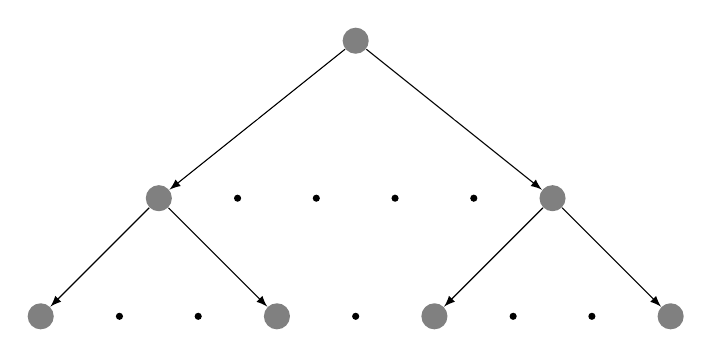
\begin{tikzpicture}[>=latex]
 \tikzstyle{every node} = [circle,fill=gray]
 \node (a) at (2.5,2) {};
 \node (b) at (0,0) {};
 \node (c) at (5,0) {};
\node (d) at (-1.5,-1.5) {};
 \node (e) at (1.5,-1.5) {};
 \node (f) at (3.5,-1.5) {};
 \node (g) at (6.5,-1.5) {};
\draw [->] (a) -- (b) node[pos=.5,sloped,above,fill=white] {};;
 \draw [->]  (a) -- (c)node[pos=.5,sloped,above,fill=white] {};;
 \draw [->] (b) -- (d);
 \draw [->] (b) -- (e);
 \draw [->] (c) -- (f);
 \draw [->] (c) -- (g);
 \fill[black] (1,0) circle (0.3ex);
 \fill[black] (2,0) circle (0.3ex);
 \fill[black] (3,0) circle (0.3ex);
 \fill[black] (4,0) circle (0.3ex);
 \fill[black] (-0.5,-1.5) circle (0.3ex);
 \fill[black] (0.5,-1.5) circle (0.3ex);
 \fill[black] (4.5,-1.5) circle (0.3ex);
 \fill[black] (5.5,-1.5) circle (0.3ex);
 \fill[black] (2.5,-1.5) circle (0.3ex);
\end{tikzpicture}
\end{center}
\caption{Mapping to  random variables in a node with data }
\label{fig:map}
\end{figure}


\begin{figure}[h]
\begin{center}
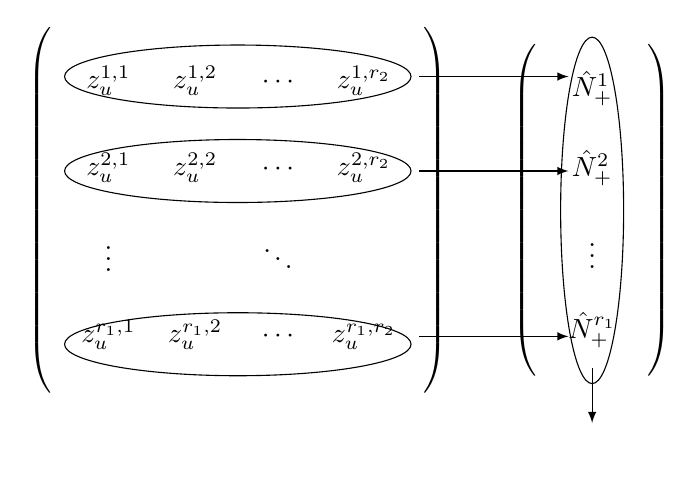
\begin{tikzpicture}[>=latex]
 \matrix (A) [matrix of math nodes,nodes = {node style ge},left delimiter  = (,right delimiter = )] at (0,0)
             {
 z_u^{1,1} & z_u^{1,2} & \cdots & z_u^{1,r_2} \\
 z_u^{2,1} & z_u^{2,2} & \cdots & z_u^{2,r_2} \\
 \vdots & & \ddots \\
 z_u^{r_1,1} & z_u^{r_1,2} & \cdots & z_u^{r_1,r_2} \\
};
\matrix (B) [matrix of math nodes,nodes = {node style ge},left delimiter  = (,right delimiter = )] at (4.5*\myunit,0)
             {
  \hat{N}_+^1 \\
  \hat{N}_+^2 \\
  \vdots \\
  \hat{N}_+^{r_1} \\
};
\draw  (0,1.7) ellipse (2.2cm and 0.4cm);
 \draw [->] (2.3,1.7) -- (4.2,1.7);
\draw  (0,0.5) ellipse (2.2cm and 0.4cm);
 \draw [->] (2.3,0.5) -- (4.2,0.5);
\draw (0,-1.7) ellipse (2.2cm and 0.4cm);
 \draw [->] (2.3,-1.6) -- (4.2,-1.6);
\draw (4.5,0) ellipse (0.4cm and 2.2cm);
 \draw [->] (4.5,-2) -- (4.5,-2.7);
\node at (4.5,-3) {};
\end{tikzpicture}
\end{center}
\caption{Estimating  and }
\label{fig:estimate}
\end{figure}


\begin{algorithm} 
  \caption{Algorithm run by node }{\label{alg:f2}}
  \begin{algorithmic}[1] 
    \REQUIRE , independent maps  
    \STATE ,  
    \STATE For each   is chosen randomly
    and independently according to 

\STATE Depending on the information spreading algorithm, node 
    receives information from node  at time  On
    receipt of this information it updates as follows:

\STATE Let  
    \STATE    
  \end{algorithmic}
\end{algorithm}


The mapping of the elements of  using random maps  are
4-wise independent in \cite{Alon96}. However, in our setting we can
use independent random maps because we are not trying to optimize the
number of bits stored per node. Rather, we are trying to optimize the
number of bits transmitted per processor. The random maps can be
thought of as global randomness shared by all the nodes.

\subsection{Error Analysis}
\label{sec:err-analysis}

Let us examine the properties of  obtained in
Algorithm~\ref{alg:f2}. If  is exactly known then
from Theorem~\ref{thm:ams-F2} the estimate of , defined as
, can be written as:

From Theorem~\ref{thm:ams-F2}, we know that 



However, we do not know, rather cannot know,  exactly for any
. In our algorithm,  is a random variable that depends on
the random map . Steps 3, 4 serve the purpose of estimating
 for the maps in Step 1, under the assumption that Step 3 has
taken place without any error.  However, recall that in point-to-point
as well as random planar networks, Step 3 itself uses randomness.

\textbf{Error in Step 3 for point-to-point networks:} We say that an
error has occurred in Step 3, if  such
that . Therefore, the probability of error is
bounded by 

\textbf{Error in Step 3 for random planar networks:} We say that an
error has occurred in Step 3, if . Therefore, the
probability of error is bounded by 

Assuming no error takes place in Step 3, we now analyze the error in
. To finally bound the overall error, we trivially
combine errors coming from different steps in the algorithm.

Recall that  is an exponential random variable.
 Assuming  is correct at time , let us
define 
Conditioned on  we can use Chernoff bound analysis to show
that for any constant 

This can be written as

where  and 


Writing  i.e.,  is the estimate of
 and expanding  we have



If 
then  can be upper bounded as:

where  Similarly
we can lower bound  as:

Combining all the three error probabilities i.e.,  
 corresponding to  maps, information spreading algorithm
and exponential random maps respectively, we get, 

Note that  depends on  and  which
can be chosen arbitrarily small. Also  and  depend on
 and  respectively. Thus these
can also be made arbitrarily small by suitably choosing  and
  can also be made arbitrarily small by suitably choosing
 

The space analysis for each node is fairly standard. We include it
here for the sake of completeness. Each node transmits a vector of
length . Each entry of this vector is an exponential random
variable. Let us assume that  bits suffice to store the exponential
random variables.\footnote{Then  in the algorithm can be
  represented using  bits.} When node  receives the vector of
 it computes the coordinate-wise minimum of the -element
vector. Only this minimum is stored at every node and transmitted at
each time the node is activated. This suffices because the ``min''
function is unaffected by the sequence in which the different nodes
are heard and also if a node is heard multiple times.  If  bits
suffice for storing exponential random variables, then each node
transmits  bits.  is determined below by suitably
truncating and quantizing the  which are exponential
random variables. 

We will show below that  bits of precision suffice to store
 This will allow  to be estimated within the same
factor of approximation with an additional small error. We thus modify
only Step~2 in Algorithm~\ref{alg:f2} as follows:

\begin{algorithm}
  \caption{Modified step 2 of Algorithm~\ref{alg:f2} with quantized
    random variables}{\label{alg:quant}} 
  \begin{algorithmic}[2a] 
    \STATE For  generate  by the
    following rule until  
    
  \item[] Uniformly quantize  using  bits.
  \end{algorithmic}
\end{algorithm}
The other steps of the Algorithm~\ref{alg:f2} remain unchanged.  If
the maximum relative error in estimating  due to truncation is
 and  and  are both chosen as  then the
estimate of  is, following the analysis of \cite{Ayaso08},

Here,  and  This means that in gossip networks at each step a node will transmit  bits. 
Further this also tells us that the each slot
of the slotted Aloha protocol should be  bit
periods.

We have thus proved Theorem~\ref{thm:main}. 

\subsection*{Percolating RPRN}

Let us now consider the computation of the estimate of  in
percolating RPRN except that a fixed fraction of the data is missing,
i.e.,  of the nodes have participated in the
computation of  Let  be the second frequency
moment calculated from  nodes.  Let  be arranged in
the descending order as .  It
is easy to see that the difference between  and 
will be maximized when the nodes that are removed had value
. Therefore,

If 

If , then similar calculations can be performed to
get the same bound. Let  be the output of
Algorithm~2 applied on  nodes. Then by
Theorem~\ref{thm:main} we know,
  
Using equations \ref{eq:f2a} and \ref{eq:f2b}, we get,

Equation \ref{eq:f2percolation} is applicable to the networks which
operate in percolation regime where a constant fraction of the nodes
do not take part in function computation. Therefore, we have the
following corollary,
\begin{corollary}
  \label{corollary:percolation}
  For all constants , there exist  so that there is a randomized algorithm that runs in time  uses  bits of transmission per step and computes an estimate of
  , say , as 
  . Here  is the time
  needed by the spread algorithm and  is the fraction of the
  nodes which are not in the giant
  component.
\end{corollary}

\subsubsection{Second frequency moment using bottom- sketch}
\label{sec:bottom_sketch}

In Algorithm~\ref{alg:f2}, for each node  and ,
 is mapped to  independent random variables. Let   denote
the vector computed by the node  after time  Note that each
 is an  sized vector each element of which is the minimum
of  independent exponential random variables.  is also known
as mins sketch in the literature \cite{Cohen07}. Recall from
Section~\ref{sec:err-analysis} that each  is an
exponential random variable with mean  and thus is used to
estimate  Recall, , therefore it is
asymptotically very small. However, in practice, reducing it to a
small constant will help in reducing the amount of randomness used by
the algorithm, and may help in bringing down the number of bits
transmitted per node.

We observe that  can be reduced to . This certainly helps in
reducing the number of random maps used per node. However, because of
the manner in which the final estimate is computed, we do not see any
way of saving the number of bits transmitted per node. We use
\emph{bottom- sketch} as defined in \cite{Cohen07}. For each , we map  to a single exponential random
variable . For a fixed , arrange 's in a
non-decreasing order, say . It is shown in \cite{Cohen07} that using  smallest
values, a good estimate can be computed.  Therefore, in our case it
will suffice if each node knows these  minimum values.  Each node
can do this by keeping track of the  smallest values seen so far
for each . This can be done by the following book keeping: Node 
holds a vector  for each
. Node  communicates the vector  to node
 and updates its vector by appropriately inserting the values from
 to get the first  minimum values available in the network
for each  At the end, for each  we have  representing the  lowest values of the
network. To summarize, each node can estimate  by generating
only one exponential random variable instead of  independent
random variables. However, to compute the bottom- sketch for
estimating , each node transfers  numbers, i.e.,
 bits of transmission per processor.

\section{Algorithm for Higher Frequency Moments}
\label{sec:Fk}

In this section we present an algorithm to compute frequency moments
 for all  In the data streaming literature, many
algorithms are known for computing  (See for example
\cite{Alon96,Coppersmith04,Ganguly04}.) In \cite{Alon96}, sampling is
used for estimating  for . For the special case of
, they give a sketching algorithm as shown in
Algorithm~\ref{alg:f2_stream}. On the other hand,
\cite{Coppersmith04,Ganguly04} use sketching algorithms for estimating
. The map  in Algorithm~\ref{alg:f2_stream} can be thought
of as a map from the input alphabet to the square roots of unity. A
possible generalization of this for  is a map from the input
alphabet to -th roots of unity. In \cite{Ganguly04} it was proved
that maps from the input alphabet to --th roots of unity can be
used for estimating  In order to estimate  in our setting,
we use a combination of random maps to --th roots of unity and
exponential random variables. Our primary observation is that Fact
\ref{fact_exp} helps us compose exponential random variables with the
maps to -th roots. This composed map in turn helps in estimating
 for  in all the three models of distributed networks.
In order to explain the central idea used in estimating  , we give a simplified version of our original algorithm:

\begin{algorithm} 
  \caption{Algorithm for higher frequency moments run by node
    }{\label{alg:fk}} 
  \begin{algorithmic}[1] 
    \REQUIRE 
    \hspace*{0.5cm} where
      
    \STATE    
    \STATE If  then for  
    
    \STATE Depending on the information spreading algorithm, node 
    receives information from  node  at time step 
    On receipt of this information it updates as follows:  
    
    \STATE  
    \STATE 
  \end{algorithmic}
\end{algorithm}

Note the similarity between Algorithm~\ref{alg:fk} and
Algorithm~\ref{alg:f2}. The above algorithm is overly simplified.  It
was observed by \cite{Ganguly04} that sum of 's when raised to
power  has expectation equal to , however its variance is very
large. This problem was resolved by using a bucketing strategy. For
each node ,  is mapped to one of  buckets
using  different maps: . (In our setting we can use
independent random maps because we are not trying to optimize the
amount of bits stored per node. We only try to optimize the number of
bits transmitted per node. The random maps can be thought of as global
randomness shared by all the nodes.) It was proved that  \cite{Ganguly04}.

The error analysis of the algorithm can be done in the same way as
done for  in Section \ref{sec:err-analysis}. It can be shown that

where  is a function of  and errors due  and
exponential random variables.

Similar to the result of  in Section \ref{sec:err-analysis}, 
is a function of  and errors due to  and
exponential random variables. As seen earlier,  can be made
arbitrarily small by controlling the errors due to the random maps and
similarly  can be made arbitrarily small by choosing 
appropriately. Proceeding on the lines of proof of Theorem~\ref{thm:main} we get Theorem~\ref{thm:Fk} from here.

\section{Discussion}
\label{sec:dis}
\begin{itemize}

\item In this paper we have considered one-shot computation of 
  For random planar networks, it is also of interest to develop
  algorithms to compute  for the sequence of  the data
  vector. In this case the computation of  for the different
  elements of the sequence will be pipelined. The techniques of
  \cite{Kamath08,Iyer11} easily extend to this case.

\item Sketching is a commonly used technique in dealing with massive
  data sets.  It involves mapping the given data from a large alphabet
  into a relatively smaller alphabet preserving the relevant
  properties. Let  be a function and let  denote a map used by a sketching
  algorithm to compute . (Note, ).  For ,
  let  denote the number of elements mapped to  under
  the mapping .  Suppose for every input ,  can be estimated
  using  then we
  call  to be \emph{sketch type sensitive.}  That is if  is
  sketch-type sensitive,  essentially depends on a type-vector,
  i.e., a vector of length , with each entry  in
  the vector corresponding to the number of elements of the original
  alphabet mapped to .   is one such function. As noted in
  Section \ref{sec:F2}, .  In fact ,  is sketch type sensitive. We believe that our techniques
  can be used for estimating any sketch type sensitive function.

\item We compute the estimate of the scaled version of , i.e.,
  . It will be interesting to estimate  itself. Also, in
  our algorithm, we assume that all nodes know sketching functions
  's.  An algorithm that does not assume such shared
  randomness will be an improvement over our algorithm.

\item This work shows that the techniques developed for space
  efficient algorithms to compute functions of streaming data can be
  used to reduce the communication in distributed computing of
  functions of distributed data. This connection needs to be explored
  further.
\end{itemize}

\bibliography{function-computation}
\bibliographystyle{plain}
\end{document}
